\documentclass[a4paper,10pt]{article}
\usepackage[utf8]{inputenc}
\usepackage{amsmath, amsfonts, graphicx}
\usepackage{hyperref, indentfirst}
\usepackage{bbold}
%opening
\title{$\mathbb{RP^2}$ and photos}
\author{}
\newcommand{\diag}{\mathop{\mathrm{diag}}}
%\vspace{-15ex}
\date{}


\begin{document}
\maketitle
\section{Introducrion}

In the previous posts we deduced the projection formula for cameras, realized that the photo can be modeled as a chart on $RP^2$ and introduced some fundamentals of real (complex) projective spaces of arbitrary dimensions. 

In this post we will talk specifically about 2-dimensional projective spaces and the related photo images. 

As it was discussed earlier, the projective space does not fully model the camera  projection as it identifies opposite rays passing through the optical center of  the camera. However, we chose to use it, because most cameras are not able to make photos of two opposite directions simultaneously and this choice drastically simplifies the math. 

It is important to bare in mind, that while modeling the photo images as charts of a projective space, we are interested in that one chosen chart only (because that what our photo is). Hence, all theorems/relations/concepts/formulae which are true for projective spaces globally will be true for any chart, however, not all claims which are true locally (for a single chart) should even make sense for the entire $\mathbb{RP}^2$ manifold. For example, as we will see below, one can have ``parallel'' lines on a chart, however for the whole projective space the idea of parallelism is not even defined.

To summarize things; we have the world coordinate system $(x_1, x_2, x_3)$ with $x_3$ axis coinciding with the principal axis of the camera lens. We also have coordinates on photo $(\xi_1^{(3)}, \xi_2^{(3)})$ which are related to the world coordinates as follows:

\begin{equation}
 \xi_1^{(3)} = \frac{x_1}{x_3}, \quad\xi_2^{(3)} = \frac{x_2}{x_3}.\label{photochart}
\end{equation}


\section{Lines on photos }

In the previous post we have understood that the set of (hyper)planes passing through the origin form the dual projective space. In case of $\mathbb{R}^3$ and corresponding $\mathbb{RP}^2$ we talk about ordinary 2-dimensional planes:
\begin{equation}
 \sum\limits_{i=1}^3 a_i x_i \equiv a\cdot x= 0. \label{plane}
\end{equation}
The projection of a plane $a$ on the chart \eqref{photochart} is a line. Indeed, dividing the equation \eqref{plane} by $x_3$ gives:

\begin{equation}
 a_1 \xi_1^{(3)} + a_2 \xi_2^{(3)} + a_3= 0,
\end{equation}
which is the equation of an arbitrary line on a plane.
Here and further we will refer to planes $a$ as "lines" meaning their projection on the  chart. However, we should always keep in mind that not all planes of $\mathbb{R}^3$ have their projection on the chart. In particular, the plain 
\begin{equation}
n^{(\infty)} = (0,0,1), \quad \text{or} \quad x_3 = 0\label{z0}
\end{equation}
does not project on the chart \eqref{photochart} and therefore cannot be referred as a "line". In the science of Computer Vision they call it a "line at infinity" (hence the superscript).

Two lines $a$ and $b$ on $\mathbb{RP}^2$  are parallel on the chart  \eqref{photochart} if 
\begin{equation}
(a\times b )\cdot n^{(\infty)} = 0, \quad \label{parallel}
\end{equation}
Alternatively, the lines on $\mathbb{RP}^2$ intersect in the point(in homogeneous coordinates)
\begin{equation}
x = a \times b.\label{intersectionpoint}
\end{equation}

In the language of lines and planes in $\mathbb{R}^3$ this can be interpreted as follows. Obviously, any two planes passing through the origin intersect. The intersection of the planes is the line passing through \eqref{intersectionpoint} and the origin. If the intersection line lies in the plane \eqref{z0} then the projections of the planes on the chart \eqref{photochart} are parallel.

The same result in the language of lines on the charts of $\mathbb{RP}^2$ is interpreted as  follows. The invariant form of \eqref{intersectionpoint} shows that, generally speaking, all lines on $\mathbb{RP}^2$ intersect and the intersection point in homogeneous coordinates is given by \eqref{intersectionpoint}. However if the condition \eqref{parallel} holds, then the intersection point is not  present on the considered chart. They say that on given chart two parallel lines intersect at the line at infinity $n^{(\infty)}$.

Now let us consider the most generic invertable transformation ({\it homography}):
\begin{equation}
x' = H x, \quad \det H \neq 0. 
\end{equation}

Obviously the line $a$ under this transformation  is "moving in the opposite direction"
\begin{equation}
a'=H^{-T}a\label{cotransform}
\end{equation}

Now, let two lines $a$ and $b$ be parallel, i.e. satisfy \eqref{parallel},  and let $H$ be a homography such that

\begin{equation}
H^{-T} \cdot a,b,n^{(\infty)}  \neq \alpha n^{(\infty)} , \quad \forall \alpha \in \mathbb{R}
\end{equation}

 It is clear that the condition $\eqref{parallel}$ is not invariant under the transformation \eqref{cotransform}. Namely,

\begin{equation}
n^{(\infty)} \cdot (a'\times b')   \neq 0
\end{equation} 
 and, hence, the transformed lines $a'$ and $b'$ intersect in the point (see\eqref{intersectionpoint}):

\begin{equation}
x' = a' \times b'
\end{equation}

It is easy to show that 
\begin{equation}
(H^{-T}n^{(\infty)}) \cdot x'  = 0
\end{equation}
and, therefore, the point of $\mathbb{RP}^2$ $x'$ on the chart \eqref{photochart} lies on the line $H^{-T}n^{(\infty)}$. 

This result is illustrated in Figures \ref{fig:3dcart} and \ref{fig:drawed}

\begin{figure}[h]
\centering
 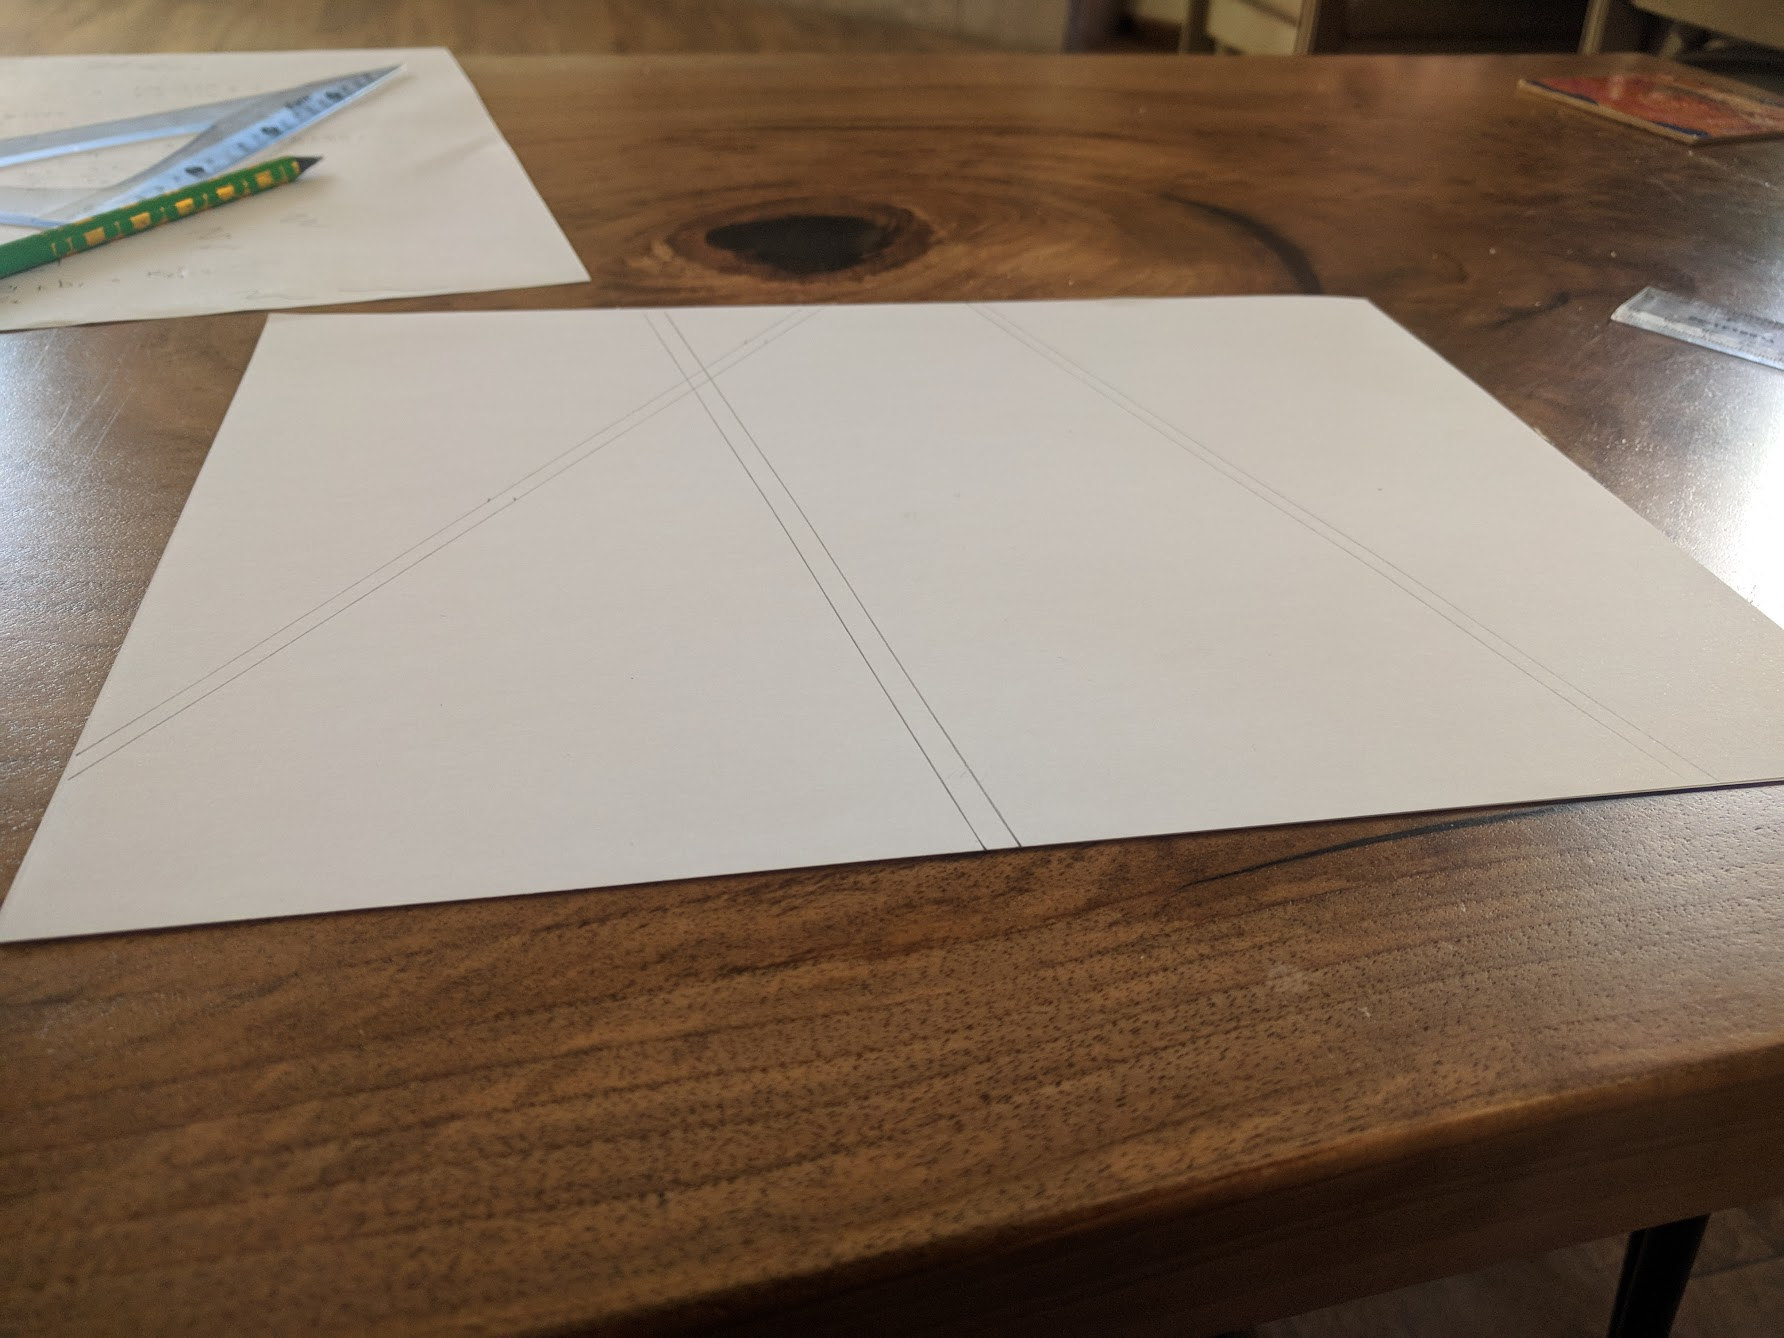
\includegraphics[width=0.6\textwidth]{../../images/parallel.jpg}
 \caption{Parallel lines taken from an arbitrary perspective. }
 \label{fig:3dcart}
\end{figure}

\begin{figure}[h]
\centering
 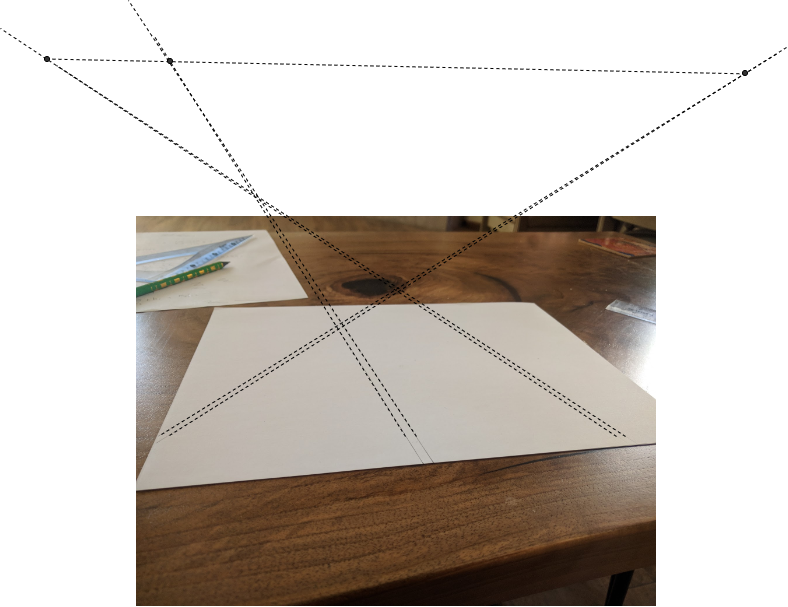
\includegraphics[width=0.7\textwidth]{../../images/parallel.png}
 \caption{The parallel lines intersect on the line at infinity. }
 \label{fig:drawed}
\end{figure}

Note, that while the plane $n^{(\infty)}$ does not have a projection on the chart \eqref{chart} the projection of the  transformed line $H^{-T}n^{(\infty)}$ is well defined. In other words, a generic {\it homography} is a linear automorphism which moves the line at infinity to the chart. 
\begin{thebibliography}{1}
\bibitem{mhopkins} Hopkins M.J. (1989) Minimal atlases of real projective spaces. In: Carlsson G., Cohen R., Miller H., Ravenel D. (eds) Algebraic Topology. Lecture Notes in Mathematics, vol 1370. Springer, Berlin, Heidelberg
\end{thebibliography}


\end{document}


